\section{Orbital Stabilization}
\showtoc

\subsection{Orbital Stabilization with Control Lyapunov Functions}
\begin{frame}
  \frametitle{Motivation}
  \begin{block}{Main Question}
    Can we use an understanding of energy exchange to improve global stability properties of periodic orbits in mechanical systems?
  \end{block}

  \begin{block}{Observations}
    \begin{itemize}
    \item Numerous control design schemes exist for stabilizing mechanical systems to periodic orbits.
    \item Some controllers produce good behavior locally but lack robustness.
    \item Periodic orbits have associated energy functions with level sets which are invariant under the orbits.
    \end{itemize}
  \end{block}
\end{frame}


\begin{frame}[t]
  \frametitle{Overview}
  \only<1>{
    \begin{block}{Setup}
      Consider the control system 
      \begin{align*}
        \dot x = f(x) + g(x) u(x).
      \end{align*}
      Assume there exists a control law ${\bar u}(x)$ which creates a limit cycle in the closed-loop dynamics,
      \begin{align*}
        {\bar f}(x) = f(\q, \dq) + g(\q) {\bar u}(\q, \dq).
      \end{align*}
      Also assume there exists an energy function $E_{c} : T\ConfigurationSpace \to \R$ which is conserved, i.e., $E_{c}(\q, \dq) \equiv E_{0}$, on the limit cycle.
    \end{block}
  }

  \only<2>{
    \begin{block}{Main Idea}
      Add robustness to a periodic behavior by imposing convergence on an energy function to a level set which is known to be invariant under the system dynamics.
    \end{block}
    
    \begin{block}{Control Objective}
      Choose control input $\mu(\q, \dq)$ such that $\| \mu(\q, \dq) - {\bar u}(\q, \dq) \|$ is minimized and $E_{c}(\q(t), \dq(t)) \to E_0$ as $t \to \infty$.
    \end{block}

    \begin{block}{Exponential Convergence}
      To achieve exponential stabilization, $E_{c}(x(t))$ should satifisy
      \begin{align*}
        E_{c}(\q(t), \dq(t)) \leq E_{c}(\q(t_{0}), \dq(t_{0})) e^{-\beta t} \mbox{ for } t \geq t_{0}, \beta > 0.
      \end{align*}
    \end{block}
  }
\end{frame}

\begin{frame}
  \frametitle{Control Lyapunov Functions}
  A \blue{control Lyapunov function} $V : X \to \R$ which satisfies
  \begin{align*}
    &c_{1} \| x \|^2 \leq V(x) \leq c_{2} \|x\|^2,\\
    &\inf_{u \in U} L_f V(x) + L_g V(x) \, u + c_{3} V(x) \leq 0
  \end{align*}
  for $c_{1}, c_{2}, c_{3} > 0$ exhibits exponential convergence.
\end{frame}

\begin{frame}
  \frametitle{Energy Shaping}
  Consider a conserved energy function $E_{c}(x)$. For an exponentially stablilzing CLF, we seek $\mu(x)$ such that
  \begin{align*}
    L_f V(x) + L_g V(x) \, \mu(x) + \epsilon V(x) &\leq 0.
  \end{align*}
  Choosing $V(x) = \eta^2$ with $\eta(x) = E_{c}(x) - E_{0}$, we obtain
  \begin{align*}
    2 \eta(x) \left(L_f \eta(x) + L_g \eta(x) \, \mu(x) \right) + \epsilon \eta^2(x) \leq 0.
  \end{align*}
  We can relax this condition by augmenting the optimization space with $\delta \in \R$ and requiring
  \begin{align*}
    2 \eta(x) \left(L_f \eta(x) + L_g \eta(x) \, \mu(x) \right) + \epsilon \eta^2(x) \leq \delta(x).
  \end{align*}
\end{frame}

\begin{frame}[t]
  \frametitle{Quadratic Program Formulation}
  The linear form of the CLF condition suggests
  \begin{align}
    \nonumber
    (\delta^*(x), \mu(x)) = \argmin_{v = (\delta, u)}  \, & v^T \! H \, v + h^T(x) v\\
    \label{clf} \tag{clf}
    \mbox{s.t. } & \Aclf(x) \, v \leq \bclf(x)%\\
    %\label{lim} \tag{lim}
    %& \Alim v \leq \blim
  \end{align}
  where \eqref{clf} imposes the control Lyapunv function. To encode the dynamics of the system under control input ${\bar u}(x)$, select
  \begin{align*}
    H = \left(\begin{array}{c c}\nu & 0\\ 0 & I\end{array}\right), & \quad
      h(x) = \left(\begin{array}{c} 0\\ -2 \, \bar u(x) \end{array}\right),\\
      \Aclf = \left(\begin{array}{c c}
        -1 & 2 \eta(x) \, L_{g} \eta(x)
      \end{array}\right), & \quad
      \bclf = -\epsilon \eta^{2}(x) - 2\eta(x) \, L_{f} \eta(x).
  \end{align*}
  with positive weighting coefficient $\nu \in \R$.
\end{frame}

\begin{frame}[t]
  \frametitle{Example: Cart with Spring}
  \only<1>{
   \begin{figure}
      \centering
      \def\svgwidth{0.8\columnwidth}
      \input{figures/cart_spring.eps_tex}
      \caption{A single coordinate, $x \in \R$, can model a cart with mass $M$ connected to a wall by a spring of stiffness $K$.}
    \end{figure}
  }

  \only<2>{
    Consider the Lypaunov candidate function
    \begin{align*}
      V(x, \dot x) = (E(x, {\dot x}) - E_{0})^{2}
    \end{align*}
    where $$E(x, {\dot x}) = \frac{1}{2} M {\dot x}^2 + \frac{1}{2} K x^2.$$
    Differentiation gives
    \begin{align*}
      {\dot V}(x, {\dot x}) = 2\left(E(x, {\dot x}) - E_{0}\right) {\dot E}(x, {\dot x})
    \end{align*}
    Under control input $u$,
    \begin{align*}
      {\dot E}(x, {\dot x}) =  L_{f}(x, {\dot x}) + L_{g} E(x, {\dot x}) u.
    \end{align*}
  }

  \only<3>{
    The Lyapunov function $V(x)$ in
    \begin{align*}
      \epsilon V(x, {\dot x}) + 2\left(E(x, {\dot x}) - E_{0}\right) \left(L_{f} E(x, {\dot x}) + L_{g} E(x, {\dot x}) u \right) \leq 0
    \end{align*}
    includes $u$ and is called a control Lyapunov function. The Lie derivatives are
    \begin{align*}
      L_{f} E(x, {\dot x}) &= \pd{E(x, {\dot x})}{x} {\dot x} + \pd{E(x, {\dot x})}{{\dot x}} \left(-\frac{K}{M} x\right)\\
      &= K x \dot x - K x {\dot x} = 0,\\
      L_{g} E(x, {\dot x}) &= \pd{E(x, {\dot x})}{{\dot x}} \frac{1}{M}\\
      &= \frac{K}{M} x.
    \end{align*}
  }

  \only<4>{
    Energy shaping is achieved by applying the following control law:
    \begin{align*}
      \mu(x, {\dot x}) = \argmin_{u \in \R} \, & u^T u\\
      \mbox{s.t. } & \Aclf(x, {\dot x}) \, u \leq \bclf(x, {\dot x})%\\
    \end{align*}
    where
    \begin{align*}
      \Aclf(x, {\dot x}) &= 2(E(x, {\dot x}) - E_{0}) \frac{K}{M} x,\\
      \bclf(x, {\dot x}) &= -\epsilon(E(x, {\dot x})- E_{0})^2.
    \end{align*}
    The closed form solution to the above is the \blue{min-norm controller}:
    \begin{align*}
      \mu(x, {\dot x}) = -\frac{1}{2} \epsilon \left(E(x, {\dot x}) - E_{0}\right) \frac{M}{K x}.
    \end{align*}
  }

  \only<5>{
    \begin{figure}
      \centering
      \includegraphics[width=0.8\columnwidth]{cart_spring_es}
      \caption{Energy shaping can shift the cart between energy levels. The difference is evident in the amplitude of the solution.}
    \end{figure}
  }

  \only<6>{
    \begin{figure}
      \centering
      \includegraphics[width=0.8\columnwidth]{cart_spring_es_energy}
      \caption{The transition between energy levels demonstrates exponential convergence.}
    \end{figure}
  }

  \only<7>{
    \begin{figure}
      \centering
      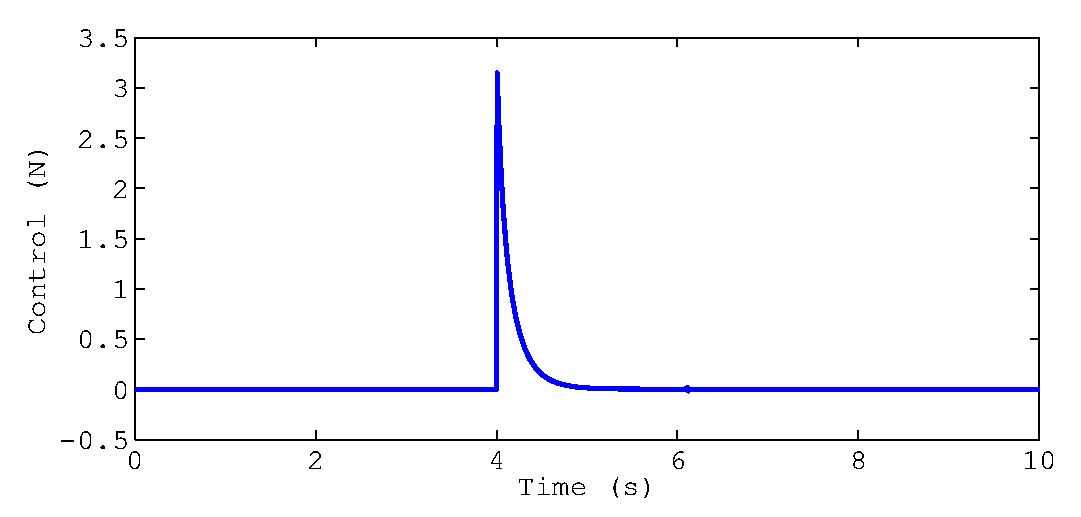
\includegraphics[width=0.8\columnwidth]{cart_spring_es_control}
      \caption{The controller applies feedback to converge to the desired energy level. Discontinuous control can be avoided with conditions on the optimization problem.}
    \end{figure}
  }
\end{frame}

